\chapter{Fundamentação teórica}
\label{cha:fundamentacao_teorica}

O desenvolvimento de software é o ato de elaborar e implementar um sistema computacional que transforme as necessidades de um utilizador ou de um mercado em um produto de software. É uma atividade essencialmente intelectual e criativa, exigindo a manipulação de uma gama muito grande de conhecimentos e informações. Além disso, os desenvolvedores de um software se preocuparem com o conteúdo e estrutura, além de deverem se preocupar também com o comportamento fazendo com o que o desenvolvimento de software seja uma atividade complexa, devendo ser realizada por especialistas munidos de técnicas que os auxiliem da melhor maneira possível.

Em 2001 um grupo de dezessete especialistas, reconhecidos pela comunidade como grandes nomes do desenvolvimento software, se reuniram para discutir sobre um crescente conjunto de métodos que vinham surgindo e decidiram usar o termo Agilismo para descrever essa nova geração de métodos \cite{AgileStory}. Na mesma reunião, eles também escreveram o Manifesto Ágil \cite{AgileManifesto}, delineando um conjunto de valores e princípios que, em resumo, trilham um caminho para a eliminação de documentação e processos desnecessários, buscando a simplicidade, com foco na geração de valor e proximidade com o cliente, além de possibilitar respostas rápidas e eficazes às mudanças. Desde então, os métodos ágeis vêm ganhando projeção e importância no cenário da produção de software.

Pode-se dizer então, que o Desenvolvimento Ágil, ou Agilismo, é um rótulo genérico para os métodos de desenvolvimento de software baseados no Manifesto Ágil \cite{BDDRodrigo}.

É importante citar que o desenvolvimento ágil sofreu grande influência de um conceito conhecido como \textit{Lean Thinking} (``pensamento enxuto"\ em português), uma linha de pensamento em gestão baseada nos princípios de \textit{Lean Manufacturing}\footnote{Os princípios de \textit{Lean Manufacturing} são originários do sistema Toyota de produção, que propôs um modo inteiramente novo de pensar a respeito de fabricação e logística de automóveis.} que se caracteriza por produção em pequenos lotes, eliminação de desperdícios, obsessão com qualidade, equipes multifuncionais praticando aprendizado contínuo, melhoria contínua de processo, sistema puxado de produção e a qualidade sendo responsabilidade dos trabalhadores como um todo \cite{BDDRodrigo}.

Uma das premissas do agilismo é que os custos de alterações sejam praticamente linear ao longo do tempo, independente do ponto em que esteja, fazendo com que a curva de custo de alterações seja semelhante à apresentada na Figura \ref{img:custo-agile}.

\begin{figure}[h]
  \center
  \caption{O custo das modificações no modelo ágil - Fonte: \cite{XPKent}}
  \includegraphics[scale=0.45]{images/custo-agile}
  \label{img:custo-agile}
\end{figure}

Isto é conseguido porque nos métodos ágeis não é feito um planejamento inicial muito abrangente. Ao invés disso, o desenvolvimento é dividido em iterações curtas (de uma a quatro semanas), onde ao início de cada uma delas é feito um novo planejamento, corrigindo o curso do projeto com base no \textit{feedback} obtido nas iterações anteriores. Para isso, a proximidade e interação do cliente com o projeto deve ser constante. Desta forma, o desenvolvimento é baseado em \textit{feedback} concreto e não em especulações sobre o futuro, fazendo com que o aprendizado permanente leve a melhorias e torne o produto final mais adequado para o seu público, além de o tornar mais simples e sem elementos extras que poderiam ser utilizados no futuro. Além disso, os testes automatizados são fundamentais para que as modificações realizadas não alterem o comportamento atual do sistema  \cite{XPKent}, dando segurança para que estas sejam feitas, além de permitir que o código melhore continuamente.

Ao utilizar métodos ágeis como \textit{eXtreme Programming} (XP) \nomenclature{XP}{eXtreme Programming} e Scrum, todas as funcionalidades do sistema são levantadas através de histórias, que são escritas pelo próprio cliente em pequenos cartões. A equipe de desenvolvimento utiliza os cartões para saber quais funcionalidades são desejadas pelo cliente. Contudo, os cartões podem acabar representando histórias que consomem muito esforço para serem implementadas. Nesse caso, a equipe divide os cartões em tarefas, que são registradas em novos cartões para serem distribuídas facilmente entre os desenvolvedores. Na Figura \ref{img:projeto_agile} é mostrada divisão de um projeto nos métodos ágeis.

\begin{figure}[h]
  \center
  \caption{Divisão de um projeto nos métodos ágeis}
  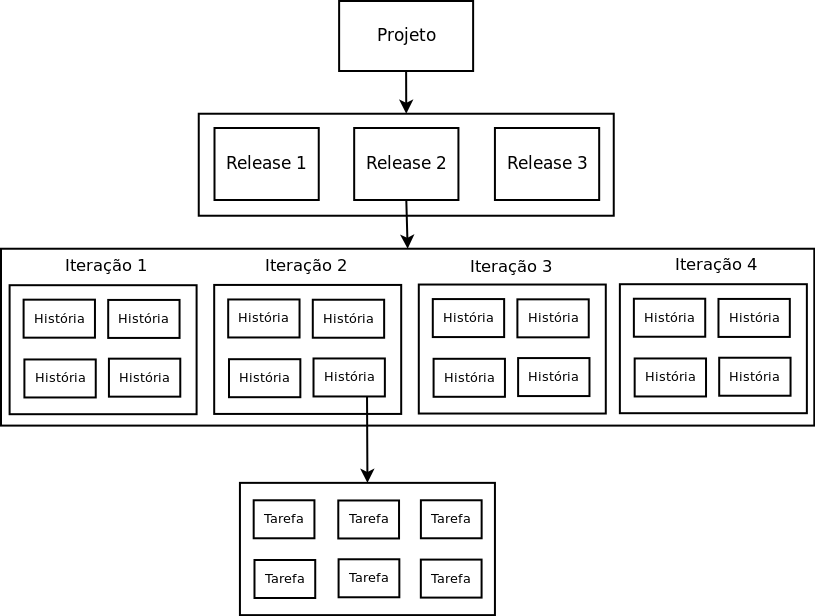
\includegraphics[scale=0.45]{images/projeto}
  \label{img:projeto_agile}
\end{figure}

No início do projeto o cliente e a equipe de desenvolvimento dividem o projeto em \textit{releases}, que são entregas de software que implementem um conjunto de funcionalidades que possui um valor bem definido para o cliente. Essas entregas são feitas de forma incremental, e em um espaço de tempo não muito longo (geralmente dois meses), para que o cliente possa começar a utilizar e obter os benefícios que elas oferecem, além de dar o \textit{feedback} necessário para que sejam feitas melhorias. Depois de definida a primeira \textit{release}, o cliente escreve as histórias que serão implementas nesta. As histórias das \textit{releases} posteriores podem ser deixadas para o futuro, pois durante o desenvolvimento de cada \textit{release} o cliente irá utilizar o software diversas vezes, o que irá influenciar as histórias das próximas \textit{release}. Durante a \textit{release} o cliente pode alterar as histórias se considerar necessário, podendo assim incorporar o aprendizado adquirido com o uso do sistema.

Uma \textit{release}, mesmo que seja pequena, representa um tempo ainda grande, pois não se deve esperar tanto tempo para ter o \textit{feedback} da utilização do software pelo cliente. Assim, ela é dividida em um conjunto de iterações, que são basicamente um pequeno espaço de tempo (geralmente duas semanas) dedicado para a implementação de um conjunto de histórias. A diferença entre uma \textit{release} e uma iteração é que na iteração o cliente não pode alterar as histórias definidas, pois a mudanças muito frequentes ao longo do trabalho da equipe de desenvolvimento prejudicam o ritmo de programação, pois confundem os desenvolvedores. No início de cara iteração é feita uma reunião para o planejamento da mesma, de modo que cliente e equipe de desenvolvimento definam as histórias que serão implementadas na iteração. Ao final de cada iteração e cada \textit{release}, o cliente tem novas histórias implementadas, ou seja, software funcionando. Dessa forma, ele poderá utilizar o sistema com as novas funcionalidades, tornando o \textit{feedback} ainda mais efetivo.

Mas para que isso seja possível, os métodos ágeis contam com um conjunto de técnicas para dar suporte a seu caráter iterativo e incremental, sendo algumas destas técnicas utilizadas para a realização do teste de software.


\section{Teste de software}
\label{sec:teste_de_software}

\textbf{TODO BEGIN}

Introduzir o que é o teste de software. Por exemplo:

Teste de Software é considerado por [Sommerville, 2007] uma técnica dinâmica de verificação e validação. Onde executamos uma implementação do software desenvolvido, apoiados em dados de teste, examinamos a saída e seu comportamento operacional para verificarmos se o seu desempenho está como solicitado/conforme necessário.

Podemos inserir uma figura do processo de desenvolvimento iterativo, dado por Sommerville na figura 17.1 da pagina 261.

\textbf{TODO END}

A maneira como o teste de software é aplicado varia de acordo com a metodologia utilizada no desenvolvimento. Tradicionalmente o teste de software é feito somente após o desenvolvimento ter sido concluído \cite{TesteSoftware, Pressman}. Já nos métodos ágeis um sentido oposto é seguido \cite{ArtOfAgileDevelopment}, sendo utilizadas técnicas como \textit{Test-Driven Development} (abordada na Seção \ref{sub:tdd}) e \textit{Behaviour-Driven Development} (abordada na Seção \ref{sub:bdd}).

O uso de estratégias nas quais a escrita dos testes automatizados é feita antes do código de implementação das funcionalidades, como TDD e BDD, não exclui o emprego de técnicas de teste de software tradicionais como classes de equivalência, análise do valor limite, análise da complexidade ciclomática e outras.

Os próximos tópicos definirão os tipos de teste utilizados no contexto do presente trabalho.


\subsection{Testes de unidade}
\label{sub:testes_de_unidade}

Testes de unidade são testes nos quais unidades individuais do sistema são testadas para determinar se estão aptas para uso. Uma unidade é a menor parte testável de uma aplicação. Em programação procedural uma unidade pode ser uma função. Já em programação orientada a objetos, uma unidade pode ser um método ou uma responsabilidade da classe. \citeonline{TesteSoftware} afirmam que neste contexto, espera-se que sejam identificados erros relacionados a algoritmos incorretos ou mal implementados, estruturas de dados incorretas, ou simplesmente erros de programação.

Para exemplificar, no Código \ref{code:unit_test_spec} é apresentado o teste de unidade para o método \texttt{Category\#name\_as\_css\_class}, cuja implementação é mostrada no Código \ref{code:unit_test}. Este método transforma o nome da Categoria em um nome de classe CSS\footnote{\textit{Cascading Style Sheets}. Mais em \url{http://pt.wikipedia.org/wiki/Cascading_Style_Sheets}}\nomenclature{CSS}{Cascading Style Sheets}, deixando todos seus caracteres em minúsculo e substituindo os caracteres / (barra),  (espaço) e - (traço) por \_ (sublinhado).

\begin{mycode}{rspec}%
{Teste de unidade automatizado para o método \texttt{Category\#name\_as\_css\_class} }{code:unit_test_spec}
# spec/models/category_spec.rb
describe Category do
  it "should return its name as a css class" do
    category = Factory.build :category, :name => "Feature"
    category.name_as_css_class.should == "feature"

    category.name = "New Feature"
    category.name_as_css_class.should == "new_feature"

    category.name = "Other-New Feature"
    category.name_as_css_class.should == "other_new_feature"

    category.name = "Study/Research"
    category.name_as_css_class.should == "study_research"
  end
end
\end{mycode}

\begin{mycode}{rspec}%
{Implementação do método \texttt{Category\#name\_as\_css\_class} }{code:unit_test}
# app/models/category.rb
class Category < ActiveRecord::Base
  def name_as_css_class
    self.name.downcase.gsub(/\/| |-/, "_")
  end
end
\end{mycode}


\subsection{Testes de integração}
\label{sub:testes_de_integracao}

\textbf{TODO: melhorar a fundamentação do teste de integração, falar realmente o que é um teste de integração, como foi feito com teste de unidade}

No contexto do presente trabalho, os testes de integração testam as integrações do código com o mundo exterior. Eles podem ser testes que se comuniquem através da rede, tenham contato com o sistema de arquivos ou deixem os limites de seu próprio processo \cite{ArtOfAgileDevelopment}.

Na Seção \ref{sec:contextualizando_tdd} será apresentado um exemplo de um testes de integração.

\subsection{Testes de aceitação}
\label{ssub:testes_de_aceitacao}

Testes de aceitação são especificações para o comportamento das funcionalidades de um sistema. Eles mostram se o sistema se comporta corretamente pela perspectiva de um usuário, sem nos dizer nada sobre como o sistema implementa esse comportamento \cite{TestDrivenKoskela}. Além disso, é verificada a integração entre as diversas unidades que interagem para prover esta funcionalidade.

Relacionando com os métodos tradicionais, os testes de aceitação implementam os casos de uso levantados na análise orientada a objetos.

No Código \ref{code:acceptance} são apresentados exemplos de teste de aceitação, utilizando BDD com a escrita em texto plano. O primeiro cenário testa a funcionalidade de clicar e arrastar as tarefas de uma posição para outra no kanban. Já o segundo cenário testa a funcionalidade de limpar a divisão \textit{Done} do kanban, ou seja, retirar do quadro todas as tarefas concluídas.

BDD e testes de aceitação serão vistos com mais detalhes na Seção \ref{sub:bdd}.

\begin{mycode}{cucumber}%
{Teste de aceitação para o registro de um contribuidor}{code:acceptance}
# features/board.feature
Feature: Use the board
  As a user
  I want use the board
  In order see, move and manipulate the taks of my project

  @javascript
  Scenario: Drag and drop a task to another board position
    Given I am an authenticated contributor
    And I have a project
    And the following tasks:
      | title  | position |
      | task 1 | Doing    |
      | task 2 | Done     |
    And I am on the projects board page
    When I drag "task 1" task to "Done" position
    Then I should see "task 1" task at "Done" position

  Scenario: Clean up Done tasks
    Given I am an authenticated contributor
    And I have a project
    And the following tasks:
      | title  | position |
      | task 1 | Doing    |
      | task 2 | Done     |
      | task 3 | Done     |
      | task 4 | Done     |
    When I am on the projects board page
    And I follow "Clean up Done"
    Then I should see "Done division was cleaned up."
    And the Done division should be cleaned
\end{mycode}


\section{Técnicas emergentes de teste de software}
\label{sec:tecnicas_emergentes_de_teste_de_software}

Nesta seção serão apresentadas, conceitualmente, as técnicas emergentes de teste de software, sendo elas o Desenvolvimento Guiado por Testes (do inglês, \textit{Test-Driven Development} - TDD), Desenvolvimento Guiado por Comportamento (do inglês, \textit{Behaviour-Driven Development - BDD}), Integração Contínua e Dublês de Teste.

\subsection{Test-Driven Development (TDD)}
\label{sub:tdd}

O \textit{Test-Driven Development} (Desenvolvimento guiado por testes) é uma técnica onde o desenvolvimento do software é guiado por \textbf{testes automatizados}, que são escritos antes de qualquer linha de código relativo a funcionalidades. Primeiro escreve-se um teste, depois escreve-se o código para passar neste teste. Em seguida, o código é refatorado para encontrar um design melhor, contando sempre com os testes existentes para que não sejam introduzidas falhas em outras partes do sistema.

Esta abordagem encoraja bom design \cite{GrowingOOByTests}, produz código testável e mantém longe a sobre-engenharia por conta de falsas suposições, pois, nos testes, é especificado o que é desejado e escreve-se o código para fazer apenas aquilo que realmente é necessário. \cite{TestDrivenKoskela, TDDbyExample, EmpiricalTDD}

\citeonline{EmergentDesign} relaciona o entendimento do problema e o fluxo natural do TDD:

\begin{citacao}
Tentar escrever um teste é uma boa maneira de testar a si mesmo sobre seu conhecimento sobre como a classe deverá funcionar antes de você escrevê-la. Esta é uma boa sequência: tenha certeza de que você entende o que você irá tentar fazer antes de você realmente tentar fazer. De fato, colocando dessa maneira, parece muito mais natural considerar os testes como Primeira Tarefa e criar o código como Segunda Tarefa. (tradução do autor)
\end{citacao}

O TDD vem sendo utilizado esporadicamente há anos, contudo, não existia um nome para identificar essa forma de desenvolver software, que no fim dos anos noventa, ganhou além do nome, uma definição. Atualmente, TDD começa a ganhar força e ser utilizada em times de grandes empresas como Google, Yahoo, Microsoft e IBM \cite{EmpiricalTDD}. O Anexo \ref{cha:a_efetividade_do_tdd} apresenta uma análise de diversos estudos sobre a efetividade de TDD na indústria e na academia.

\subsubsection{Ciclo TDD}
\label{ssub:ciclo_tdd}

Com base no trabalho de \citeonline{TDDbyExample}, o ciclo de desenvolvimento TDD é composto pelas seguintes etapas:

\begin{enumerate}
\item \textbf{Adicionar um teste}

Cada ciclo se inicia com a criação de um teste de unidade. Este teste inevitavelmente irá falhar, pois é escrito antes do código ser implementado de fato. Para escrever um teste, o desenvolvedor precisa entender claramente as especificações e requisitos da unidade. Isso faz com que o desenvolvedor tenha como foco os requisitos antes do código, o direcionando a escrever código apenas para o que é realmente necessário.

Além disso, segundo \citeonline{XPTeles}, ao se pensar e escrever o teste, está sendo feita também a análise e \textit{design} das classes do sistema.

\item \textbf{Executar todos os testes e ver se algum falha}

Todos os testes devem ser executados e o novo teste deve falhar pela razão esperada: a funcionalidade não foi desenvolvida. Isto aumenta a confiança que se está testando a coisa certa.

\item \textbf{Escrever código}

O próximo passo é escrever código \textbf{somente para que o teste passe}. O código poderá não ser perfeito, pois posteriormente ele será melhorado. O importante é que o código faça o mínimo para passar no teste. Segundo \citeonline{BDDRodrigo}:

\begin{citacao}
Enquanto código útil é um patrimônio que gera valor, qualquer código criado inutilmente é tempo desperdiçado e, no fim das contas, um fardo, que sem gerar valor algum, aumentará a complexidade geral do software.
\end{citacao}

\item \textbf{Executar os testes e ter sucesso}

Ao Executar os testes e todos eles passarem, o código possuirá todos os requisitos testados e o programador pode ficar confiante para melhorá-lo.

\item \textbf{Refatorar}

Esta é uma etapa muito importante, onde o código escrito anteriormente é melhorado. Segundo \citeonline{FowlerRefatoracao}, refatorar é reestruturar o software aplicando uma série de alterações em sua estrutura interna para torná-lo mais fácil de ser entendido e menos custoso de ser modificado, sem alterar seu comportamento observável.

Refatorar melhora o projeto do software, o torna mais fácil de entender e modificar, ajuda a encontrar falhas e ajuda o desenvolvedor a programar mais rapidamente.

Como na refatoração o comportamento do código não deve ser alterado, após refatorar e executar novamente os testes, todos eles devem passar.

\end{enumerate}

A figura \ref{img:ciclo-tdd} resume o ciclo TDD, onde as etapas 1 e 2 são representadas pelo item \textbf{teste}, as etapas 3 e 4 pelo item \textbf{codifique} e a etapa 5 pelo item \textbf{refatore}.

\begin{figure}[h]
  \center
  \caption{O ciclo TDD}
  \includegraphics[scale=0.45]{images/ciclo-tdd}
  \label{img:ciclo-tdd}
\end{figure}


\subsubsection{Design emergente}
\label{ssub:design_emergente}

No contexto em que TDD costuma ser aplicado $-$ em processos ágeis, com um ciclo de vida iterativo-incremental $-$ não é realizado um amplo \textit{design} prévio. Sendo assim, o \textit{design} evolui incrementalmente, ou seja, o \textit{design} emerge de acordo com a necessidade. Sabendo disso, uma característica extremamente importante do TDD é a facilitação ao \textit{design} emergente, que muitos consideram ser sua a principal característica \cite{EmergentDesign}.

TDD é considerada uma técnica essencial para o \textit{design} emergente porque
quando se está escrevendo um teste anteriormente ao código, o programador contempla e decide não apenas a interface do software (i.e. nomes de classes/métodos, parâmetros, tipos de retorno, lançamento de exceções), mas também o comportamento do software (i.e. resultados esperados para determinadas entradas) \cite{JanzenTDD}.

Além disso, \citeonline{EmergentDesign} constata que o ponto de vista do teste pode passar informações sobre o design, porque o teste de uma classe funciona como o primeiro cliente da classe. Com isso, a interface que o teste sugere é uma interface dirigida ao cliente, sendo assim, geralmente é mais estável.

\citeonline{DammTDD} também afirmam que o TDD faz com que as pessoas pensem mais no design em vez de codificar precipitadamente sem saber o que implementar ainda e \citeonline{XPTeles} ressalta a importância da refatoração para a evolução incremental do design:

\begin{citacao}
Ao longo das iterações, o design precisa evoluir, mas deve manter-se simples e claro para que a equipe possa fazer alterações no software a qualquer momento, com facilidade. Por esta razão o \textit{refactoring} tem um papel fundamental no design.
\end{citacao}


\subsection{Behaviour-Driven Development (BDD)}
\label{sub:bdd}

Criado em 2006 \cite{IntroducingBDD}, \textit{Behaviour-Driven Development} (Desenvolvimento guiado por comportamento) é uma técnica de desenvolvimento de software cuja amplitude se estende às atividades de design, documentação, validação e verificação, tratando-as de modo unificado \cite{BDDRodrigo}.

O Principal objetivo do BDD é ter especificações (também consideradas documentações) executáveis do sistema. Tudo que foi dito anteriormente sobre TDD vale também para BDD, mas em BDD os testes são escritos de forma mais clara e são mais facilmente lidos, pois BDD provê uma \textit{ubiquitous language} baseada no domínio do problema. Com isso, o vocabulário do problema (negócios) permeia diretamente para o código \cite{IntroducingBDD}.

\subsubsection{Ubiquitous Language}
\label{ssub:ubiquitous_language}

Uma \textit{ubiquitous language} é uma linguagem baseada no domínio do negócio, permitindo que clientes e desenvolvedores falem a mesma língua sem ambiguidade. Segundo \citeonline{BDDSolis}, o conceito de \textit{ubiquitous language} é o núcleo do BDD.


\citeonline{DDD} diz que uma \textit{ubiquitous language} é uma linguagem comum a todo o projeto, cobrindo toda acadeia de comunicação, desde conversas entre o cliente e o analista de negócios até conversas internas da equipe de desenvolvimento, chegando aos termos utilizados no código e mesmo nas estruturas de banco de dados.

Dessa forma, uma \textit{ubiquitous language} estreita a colaboração entre clientes e desenvolvedores, ao facilitar a comunicação e o \textit{feedback} \cite{DDD}.

\subsubsection{O ciclo BDD}
\label{ssub:o_ciclo_bdd}

O Ciclo BDD (também chamado de ciclo \textit{outside-in}\footnote{O ciclo recebe este nome devido à sequência que deve ser percorrida, que se inicia dos requisitos e da visão do cliente (\textit{outside}) até as entranhas dos artefatos de software (\textit{in}) \cite{BDDRodrigo}.}), apresentado na Figura \ref{img:ciclo-bdd}, tem dois níveis: unidade e aceitação. O nível aceitação é o nível mais alto, onde são escritos os testes de aceitação. Já o nível unidade é o mesmíssimo \hyperref[ssub:ciclo_tdd]{ciclo TDD} visto anteriormente. Este ciclo pode ser explicado na seguinte série de passos:

\begin{enumerate}
\item \textbf{Adicionar um teste de aceitação com foco em um cenário}

Cada ciclo se inicia com a criação de um teste de aceitação, tendo como foco um cenário que descreve um determinado comportamento de uma funcionalidade do sistema. Para fazer um paralelo com os métodos tradicionais de desenvolvimento de software, pode-se ver os cenários como casos de uso.

\citeonline{BDDRodrigo} define como que, em BDD, o foco do desenvolvedor deve estar em um único cenário por vez, e os benefícios dessa abordagem:

\begin{citacao}
Na terminologia de BDD, um cenário é um exemplo de utilização de uma dada funcionalidade. Uma funcionalidade é algo que o software deve oferecer e que possui um valor bem definido para o cliente. Em BDD, o foco dos desenvolvedores deve estar sempre direcionado à um único cenário de uma única funcionalidade por vez. Isto elimina dispersões e mantém o desenvolvedor concentrado na tarefa a ser realizada. Um desenvolvedor utilizando BDD deve encarar um novo cenário como se todos os requisitos do software fossem apenas os cenários já implementados e o atual, ou seja, não se preocupará, no momento, com as próximas funcionalidades ou cenários. Isto é importante para evitar generalizações baseadas em especulações a respeito do que o software possa eventualmente necessitar no futuro, o que aumenta a complexidade do \textit{design} sem qualquer garantia de que será realmente útil.
\end{citacao}

\item \textbf{Executar todos os testes e ver se algum falha}

Assim como no \hyperref[ssub:ciclo_tdd]{ciclo TDD}, todos os testes devem ser executados e o novo teste deve falhar pela razão pois a funcionalidade ainda não foi desenvolvida.

\item \textbf{Descer de nível}

Neste momento, deve-se descer de nível, saindo do nível de aceitação e indo para nível de unidade.

\item \textbf{Entra no ciclo TDD}

No nível de unidade, entra-se no \hyperref[ssub:ciclo_tdd]{ciclo TDD} até que todos os testes de unidade estejam passando.

\item \textbf{Retornar para o nível de aceitação}

Com todos os testes de unidade passando, retorna-se para o nível de aceitação e faz-se todos os testes deste nível passarem.

\item \textbf{Refatorar}

Neste passo, é feita a refatoração do código, da mesma maneira como é feita no \hyperref[ssub:ciclo_tdd]{ciclo TDD}.

\end{enumerate}

\begin{figure}[h]
  \center
  \caption{O ciclo BDD}
  \includegraphics[scale=0.45]{images/ciclo-bdd}
  \label{img:ciclo-bdd}
\end{figure}

\subsection{Integração contínua}
\label{sub:integracao_continua}

Em uma equipe com vários desenvolvedores, todos trabalhando na elaboração de um mesmo sistema, existe o problema de unificar as diversas alterações feitas na base de código, assegurando que a base continua consistente \cite{ImproveitCI}. Para resolver esse problema, entra em cena a Integração Contínua (IC) \nomenclature{IC}{Integração Contínua}, que além disso, tem como ponto chave dar um feedback rápido quando a base de código não está consistente.

\cite{FowlerCI} definiu a IC da seguinte maneira:

\begin{citacao}
Integração Contínua é uma prática de desenvolvimento de software onde os membros de um time integram seu trabalho frequentemente, geralmente cada pessoa integra ao menos uma vez ao dia $-$ podendo haver múltiplas integrações por dia. Cada integração é verificada por um \textit{build} automatizado (incluindo testes) para detectar erros de integração o mais rápido possível. Muitos times acham que essa abordagem leva a uma significante redução nos problemas de integração e permite que um time desenvolva software coeso mais rapidamente. (tradução do autor)
\end{citacao}

Para assegurar o rápido feedback, o tempo de execução da \textit{build} deve ser o menor possível, tentando manter sempre menor do que dez minutos \cite{FowlerCI}.

Além disso, no servidor de integração, busca-se utilizar as mesmas configurações utilizadas em produção, pois em algumas situações os testes podem estar passando em ambiente de desenvolvimento, mas o \textit{bug} estourar em produção. O intuito é eliminar a famosa frase ``Na minha máquina funciona!".

A IC é um dos pilares da agilidade, pois garante que todo o sistema funcione de forma coesa a cada \textit{build}, mesmo que sua equipe seja grande e diversas partes do código estejam sendo alteradas ao mesmo tempo \cite{CaelumCI}.

Existem duas formas de executar a integração contínua: síncrona e assíncrona.

\subsubsection{Integração contínua síncrona}
\label{ssub:integracao_continua_sincrona}

Para a utilização da integração contínua síncrona, todos os desenvolvedores devem trabalhar no mesmo espaço físico, pois deve existir uma máquina dedicada à integração. Assim, apenas um desenvolvedor integra seu código de cada vez e outros só são liberados para integrar ao serem informados do término da integração corrente \cite{ImproveitCI}.

%subsection integracao_continua_assincrona (end)


\subsubsection{Integração contínua assíncrona}
\label{ssub:integracao_continua_assincrona}

Na integração contínua assíncrona, não existe a necessidade de todos os desenvolvedores trabalharem no mesmo espaço físico. Esse modelo é ideal para a maioria dos projetos \textit{open source}, onde os desenvolvedores estão espalhados em diversas partes do mundo, pois em tais casos torna-se difícil ou impossível garantir que apenas um desenvolvedor irá integrar de cada vez \cite{ImproveitCI}.

Nesse modelo, o desenvolvedor deve assegurar que todos os testes estejam passando em sua máquina, e com essa condição atendida, pode integrar seu código ao repositório.

Além disso, um servidor de integração contínua, como o Jenkins\footnote{\url{http://jenkins-ci.org}} ou Travis\footnote{\url{http://travis-ci.org}}, deve monitorar o repositório permanentemente. Sempre que o servidor detecta modificações ele roda a \textit{build} e se encontra algum erro, envia um email para os desenvolvedores. Dessa forma, o desenvolvedor responsável deve fazer as correções o mais brevemente possível e enviá-las para o repositório.


\subsection{Dublês de Teste}
\label{sub:dubles_de_teste}

Em algumas ocasiões é difícil testar alguns componentes porque eles dependem de outros componentes que não podem ser utilizados em ambiente de teste. Estas situações podem acontecer por esses componentes não estarem disponíveis, por eles não retornarem os resultados necessários ou porque executá-los iria trazer efeitos colaterais indesejados. Em outros casos, a estratégia de testes utilizada requer que se tenha mais controle do comportamento interno do componente.

Quando se escreve um teste onde não se pode/escolhe usar componentes reais, pode-se substitui-los pelos Dublês de Teste que oferecem uma maneira de isolar as dependências ao criar os testes, permitindo a utilização de componentes falsos para cumprir os papéis de componentes reais. Com isso, elimina-se complexidade do código dos testes, pois o código de implementação dos objetos é mantido pequeno e com baixo acoplamento.

Uma outra característica da utilização de dublês é que muitas vezes fazem com que os testes sejam executados mais rapidamente, pois criam o objeto apenas em memória, reduzindo assim o acesso a disco.

Os Dublês de Teste não precisam se comportar exatamente como o componente real, devendo apenas prover a mesma API que o componente real.

\citeonline{XUnit} define cinco categorias de Dublês de Teste:

\begin{itemize}
\item
\textbf{\textit{Dummy}} geralmente apenas preenche uma lista de parâmetros e nunca é utilizado de fato.

\item
\textbf{\textit{Fake}} é utilizado para substituir uma funcionalidade real. Geralmente, o \textit{fake} implementa a mesma funcionalidade, porém de uma maneira muito mais simples. Um exemplo típico é uma base de dados em memória.

\item
\textbf{\textit{Stub}} provê respostas prontas para chamadas feitas durante os testes, geralmente não respondendo a qualquer chamada diferente
das pré-definidas.

\item
\textbf{\textit{Spy}} é um \textit{stub} que também grava algumas informações baseadas em como ele é chamado. Um exemplo pode ser um serviço de email que grava quantas mensagens foram enviadas.

\item
\textbf{\textit{Mock}} é um objeto pré-programado para receber determinado conjunto de chamadas, podendo lançar uma exceção se tais chamadas não forem feitas a ele, ou se receber outra chamada diferente das pré-programadas.

\end{itemize}

Destes cinco tipos de dublês, apenas dois serão abordados, sendo eles \textit{mock} e \textit{stub}, por serem os mais amplamente utilizados, além de serem os únicos necessários no desenvolvimento do kanban-roots.